\documentclass[12pt]{report}

\usepackage{graphicx}
\usepackage{tabu}
\usepackage{geometry}
\usepackage{minitoc} 
\usepackage{amsmath}
\usepackage{algorithm}
\usepackage[noend]{algpseudocode}
\usepackage[sorting=none]{biblatex} 
\addbibresource{reference.bib}

\usepackage{amssymb}
\usepackage{listings}
\usepackage{dirtytalk}
\usepackage{enumitem}
\setlist[enumerate]{itemsep=0mm}
\setlist[itemize]{itemsep=0mm}
\usepackage{graphicx}
\graphicspath{ {./figures/} }


%multiple columns can be created 
\usepackage{multicol}

\usepackage{xcolor}
\usepackage{subcaption}
\definecolor{codegreen}{rgb}{0,0.6,0}
\definecolor{codegray}{rgb}{0.5,0.5,0.5}
\definecolor{codepurple}{rgb}{0.58,0,0.82}
\definecolor{backcolour}{rgb}{0.95,0.95,0.92}

\lstdefinestyle{mystyle}{
	backgroundcolor=\color{backcolour},   
	commentstyle=\color{codegreen},
	keywordstyle=\color{magenta},
	numberstyle=\tiny\color{codegray},
	stringstyle=\color{codepurple},
	basicstyle=\ttfamily\footnotesize,
	breakatwhitespace=false,         
	breaklines=true,                 
	captionpos=b,                    
	keepspaces=true,                 
	numbers=left,                    
	numbersep=5pt,                  
	showspaces=false,                
	showstringspaces=false,
	showtabs=false,                  
	tabsize=2
}

\lstset{style=mystyle}


\usepackage{sectsty}
\chapterfont{\centering}
\geometry{a4paper, tmargin=1in, rmargin=1in, bmargin=1in, lmargin=1in}


\usepackage{cryptocode}



% sets roll number , name and title
\newcommand{\rollno}{2220}
\newcommand{\name}{student name}
\newcommand{\topic}{Project title}
\newcommand{\guide}{Guide name}
\newcommand{\hod}{Dr.Tonmoy Hazara}

\usepackage{fancyhdr}

\pagestyle{fancy}
\fancyhf{}

\fancyhead[RE,LO]{\topic}
\fancyfoot[RE,LO]{\leftmark}
\fancyfoot[LE,RO]{\thepage}

\renewcommand{\headrulewidth}{1pt}
\renewcommand{\footrulewidth}{1pt}


\renewcommand*\contentsname{\hfill\textbf{\textbf{\fontsize{16pt}{24pt}\selectfont TABLE OF CONTENTS}} \hfill}
\renewcommand{\bibname}{REFERENCES}
\setcounter{tocdepth}{1}

\begin{document}
\begin{titlepage}
	\begin{center}
	\fontsize{18pt}{18pt} \selectfont \textbf{Satellite To Map Image Conversion Using Deep Learning}
	\vspace*{1.4cm}

	\fontsize{13pt}{13pt} \selectfont {A Project report submitted in partial fulfillment of the requirements for the award of the degree of}
	
	
	\vspace*{0.8cm}
	\fontsize{14pt}{1cm}\selectfont\textbf{\textit{MASTER'S OF TECHNOLOGY } }
	
	\textbf{in\\}
	
	\fontsize{14pt}{1cm}\selectfont\textbf{\textit{Computer Science and Engineering}}
	
	\vspace*{0.8cm}
	by
	
	\vspace*{0.8cm}
	\textbf{Chaitanya Arora}\\
	\textbf{MIS No:222115003}\\
	\textbf{ Semester: II}
	
	\vspace*{0.4cm}
	\begin{center}
	  
\includegraphics[width=2.5in]{iiitp_logo.png}  
	\end{center}
		\vspace*{0.3cm}
	\fontsize{12pt}{0.5cm}\selectfont \textbf{Computer Science and Engineering}\\
	\vspace*{0.5cm}
	\fontsize{12pt}{12pt}\selectfont \textbf{Indian Institute of Information And Technology Pune}\\
	\vspace*{0.5cm}
	\fontsize{12pt}{12pt}\selectfont \textbf{Near Bopdev Ghat, Kondhwa Annexe, Yewalewadi, Pune, Maharashtra 411048}\\
	
	\vspace*{1.3cm}
		
\end{center}
\end{titlepage}


\pagenumbering{gobble}
\thispagestyle{plain}
\begin{center}
\fontsize{16pt}{14pt}\selectfont\textbf{BONAFIDE CERTIFICATE}
\end{center}

\vspace{0.3cm}
% Enter the title of your project in the section where it says PROJECT NAME
\fontsize{12pt}{24pt}\selectfont This is to certify  that the project report entitled   \textbf{“Satellite To Map Image Conversion Using Deep Learning”}  submitted by  \textbf{Chaitanya Arora} bearing the  \textbf{MIS No: 222115003},  in completion of his project work under the guidance of  \textbf{Dr.Rahul Dixit} is accepted for the project report submission in partial fulfillment of the requirements for the award of the degree of Master of Technology in Computer Science and Engineering in the Department of Computer Science and Engineering , Indian Institute of Information Technology, Pune, during the academic year 2022-23.


\vspace{2.5cm}


% \begin{figure}[h]
%		\includegraphics[scale=0.2]{figures/yesoda_maam_sign.jpeg}
%		\label{}
%\end{figure}


\fontsize{12pt}{20pt}\selectfont 
\noindent
\begin{tabu}{X[l] l}
 \textbf{Dr.Vaidurya Jain}\textbf{} & \textbf{Dr. Rahul Dixit} \\
 Project Guide & Project Guide\\
 Assistant Professor & Assistant Professor \\
 Department of Humanities Social Sciences and Management & Department of CSE\\
 IIIT Pune & IIIT Pune\\
\end{tabu}

\vspace{2.0cm}
\noindent
\begin{tabular}{lc}
% \fontsize{12pt}{24pt}\selectfont Project Viva-voce held on & \underline{\hspace{2in}}
\fontsize{12pt}{24pt}\selectfont Project viva-voce held on & \underline{25/04/2022}

\end{tabular}

\vspace{3.5cm}
\fontsize{12pt}{18pt}\selectfont 
\noindent
\begin{tabu} to \textwidth { X[l] X[c] }

 \textbf{Internal Examiner} & \textbf{External Examiner}

\end{tabu}

\newpage
\begin{center}
\textbf{\textbf{\fontsize{16pt}{24pt}\selectfont ACKNOWLEDGEMENT}}
\end{center}

\vspace{0.3cm}

\fontsize{12pt}{24pt}\selectfont 
This project would not have been possible without the help and cooperation of many. I would like to thank the people who helped me directly and indirectly in the completion of this project work.\par
\hspace{0.3cm}  First and foremost,\hspace{0.1cm} I would like \hspace{0.1cm}  to express \hspace{0.1cm}  my gratitude  \hspace{0.1cm}  to our beloved  \hspace{0.1cm} director,\hspace{0.3cm}  \textbf{Dr. Anupam Shukla}, for providing his kind support in various aspects. \par

I would like to express my gratitude \ to \ my project guides \ \textbf{Dr. Rahul Dixit}, Assistant Professor, Department of CSE, for providing excellent guidance, encouragement, inspiration, constant and timely support throughout this M.Tech project.\par

I would like to express my gratitude to my project guides \textbf{Dr.Vaidurya Jain}, Department of Humanities Social Sciences and Management, for providing his kind support in various aspects.\par
I would also like to thank all the faculty members in the Dept. of CSE and my classmates for their steadfast and strong support and engagement with this project. 


\addcontentsline{toc}{chapter}{Abstract}
\pagenumbering{roman}
\begin{center}
	\textbf{\textbf{\fontsize{16pt}{24pt}\selectfont Abstract}}
\end{center}
\par Conditional adversarial networks are being investigated as a general-purpose solution to image-to-image translation difficulties. These networks not only learn the mapping from input to output image, but also the loss function that will be used to train the mapping. This allows the same generic method to be applied to problems that would normally require quite different loss formulas. We show that, among other things, this method may be used to synthesise photographs from label maps, reconstruct objects from edge maps, and colourize images. Its broad applicability and ease of adoption without the need for parameter tweaking are further demonstrated. It's used to create effective losses. To put it another way, we still need to tell CNN what we want it to downplay.This is due to the fact that Euclidean distance is reduced by averaging all feasible outputs, resulting in blurring. Developing loss functions that drive the CNN to accomplish what we truly want — e.g., output clear, realistic images – is a work in progress that typically necessitates specialist knowledge. It would be ideal if we could instead give merely a high-level aim, such as "make the output indistinguishable from reality," and then the loss function appropriate for achieving this goal would be learned automatically. Fortunately, the recently suggested Generative Adversarial Networks achieve precisely that (GANs). GANs learn a loss that attempts to classify whether the output image is real or false while also training a generative model to reduce the loss. Blurry photos will not be accepted because they can be applied to a multitude of tasks that traditionally would require very different kinds of loss functions.



\\ \textbf{\textit{Keywords : }} GAN Model, CNN,RNN,LSTM, Deep Learning
%First paragraph \par
%Second Paragraph \par
%Third Paragraphy \par


\tableofcontents

\cleardoublepage
\addcontentsline{toc}{chapter}{\listfigurename}
\listoffigures

\cleardoublepage
\addcontentsline{toc}{chapter}{\listtablename}
% \listoftables

%\cleardoublepage
%\addcontentsline{toc}{Chapter}{Listing}
%\lstlistoflistings

\cleardoublepage
\chapter{ Introduction} \label{ch:intro}
\pagenumbering{arabic}

%\section{First Section}
%\subsection{WELCOME}


\subsection{Introduction}

\par Many image processing, computer graphics, and computer vision challenges can be described as "translating" an input image into a corresponding output image. A scene can be displayed as an RGB image, a gradient field, an edge map, a semantic label map, and so on, just as a thought can be expressed in English or French. We describe automatic image-to-image translation as the challenge of translating one possible representation of a scene into another, given adequate training data, in the same way that automatic language translation is defined. Despite the fact that the setting is always the same: forecast pixels from pixels, each of these jobs has traditionally been done with distinct, special-purpose gear. The purpose of this study is to create a common framework for all of these issues.

Many image processing, computer graphics, and computer vision challenges can be described as "translating" an input image into a corresponding output image. A scene can be displayed as an RGB image, a gradient field, an edge map, a semantic label map, and so on, just as a thought can be expressed in English or French. We describe automatic image-to-image translation as the challenge of translating one possible representation of a scene into another, given adequate training data, in the same way that automatic language translation is defined. Despite the fact that the setting is always the same: forecast pixels from pixels, each of these jobs has traditionally been done with distinct, special-purpose gear. The purpose of this study is to create a common framework for all of these issues.


GANs with conditions GANs aren't the first to be used in a conditional setting. GANs have been trained on discrete labels, text, and even images in previous and concurrent studies. Image prediction from a normal map, future frame prediction, product photo generation, and image generation from sparse annotations have all been solved by image-conditional models. Several other articles have employed GANs for image-to-image mappings, but they only used them unconditionally, relying on other terms (such as L2 regression) to condition the output on the input. Inpainting, future state prediction, image alteration directed by user constraints, style transfer, and superresolution are all topics covered in these publications. Each method was created with a specific application in mind. Nothing about our framework is application-specific.

Our generator and discriminator architectures are based on those used in Both the generator and the discriminator use convolution BatchNormReLu modules.
Several architectural choices for the generator and discriminator distinguish our method from previous work. Unlike previous work, we use a "U-Net"-based architecture for our generator, and a convolutional "PatchGAN" classifier for our discriminator, which only penalises structure at the scale of image patches. To capture local style statistics, a similar PatchGAN architecture was presented previously in. We show that this method works on a broader range of situations and study the impact of modifying the patch size.




\par  


\subsection{Satellite To Map Image Conversion}

\par  By using the GAN model, satellite photos can be converted to map images. Conditional adversarial networks are being investigated as a general-purpose solution to image-to-image translation difficulties. These networks not only learn the mapping from input to output image, but also the loss function that will be used to train the mapping. Image prediction from a normal map, future frame prediction, product photo generation, and image generation from sparse annotations have all been solved by image-conditional models. Several other articles have employed GANs for image-to-image mappings, but they only used them unconditionally, relying on other terms (such as L2 regression) to condition the output on the input. Not only do these networks learn the mapping from input to output image, but they also learn a loss function.


	\begin{figure}[h!]
    \centering
    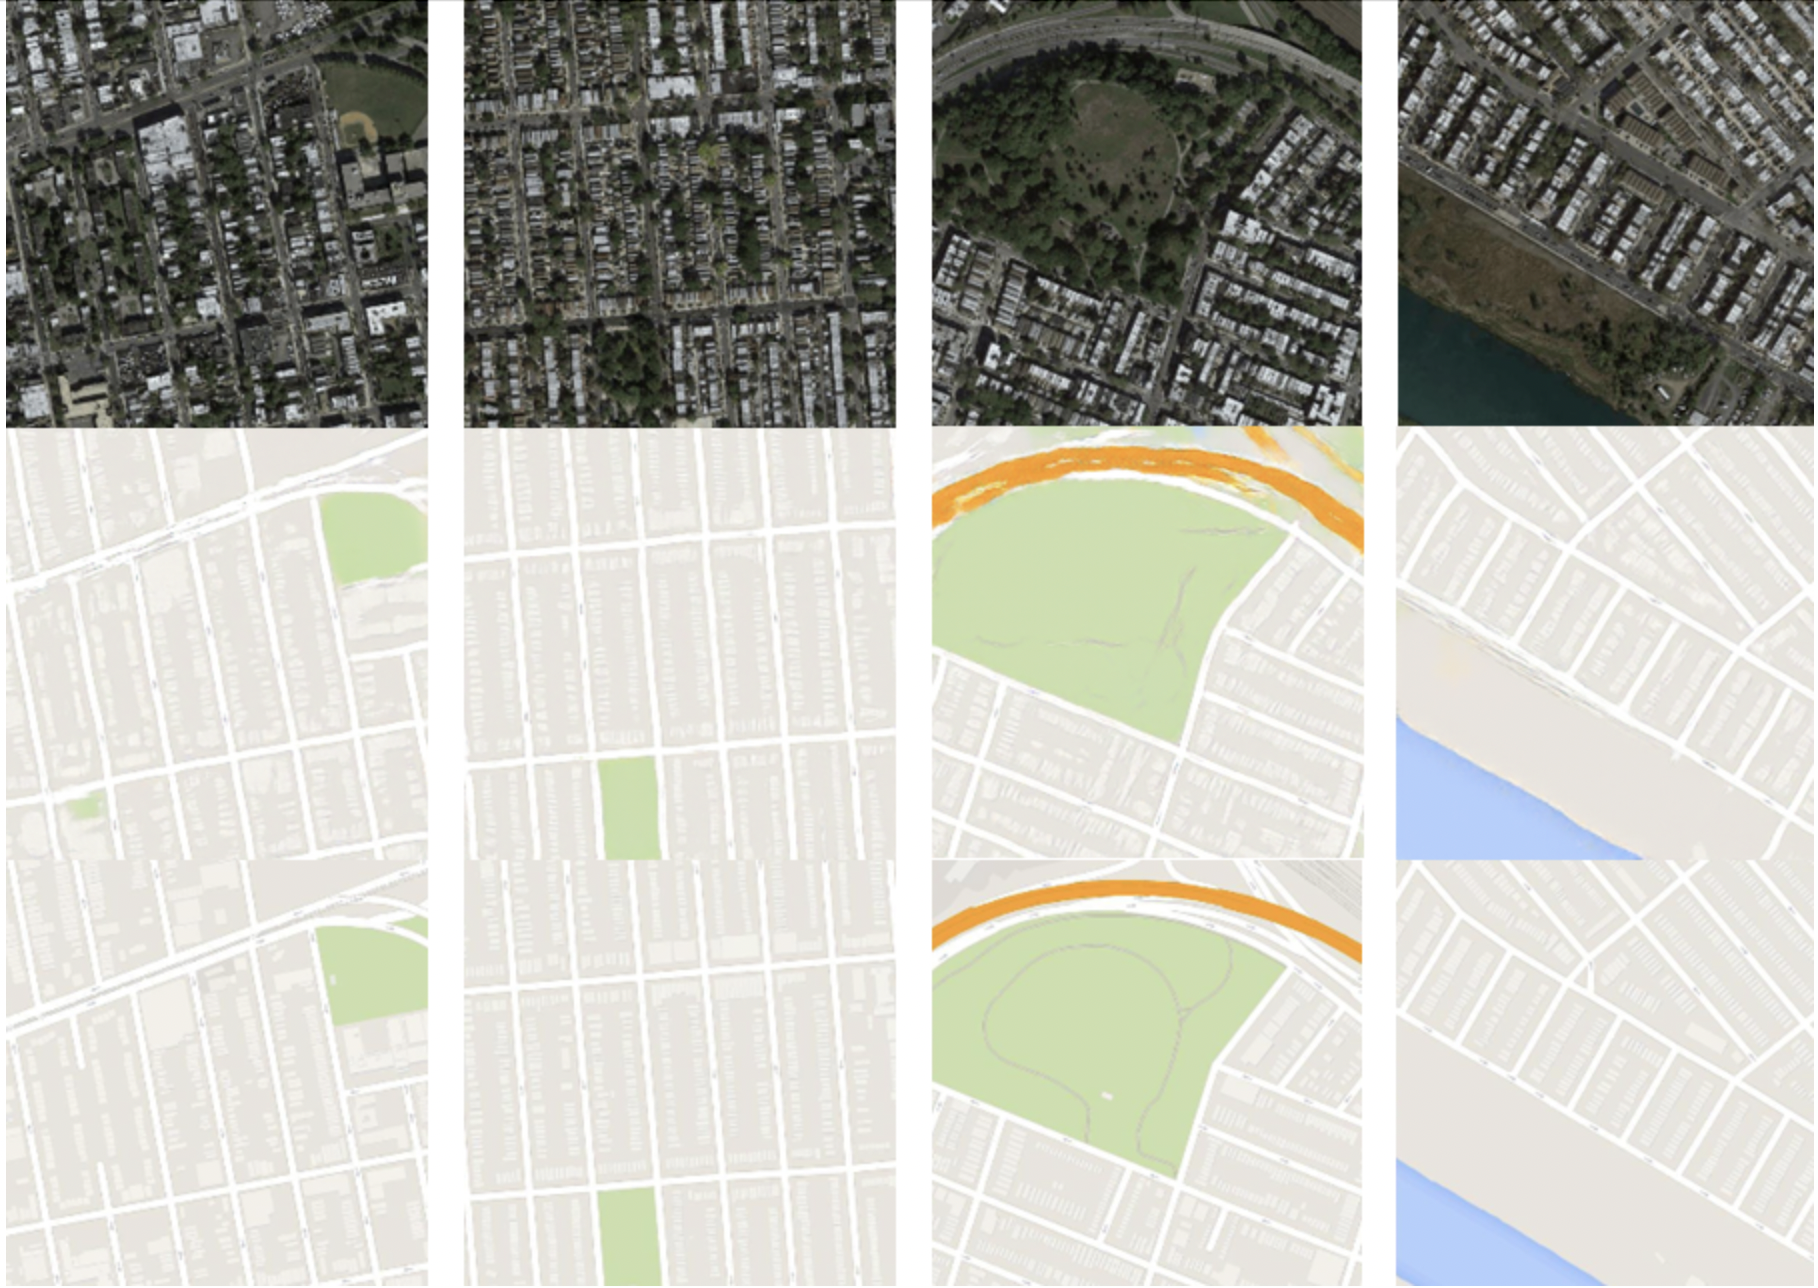
\includegraphics[width=\linewidth,height=7cm]{figures/2.png}
    \caption{ Satellite To Map Image Conversion }
    \label{fig:GAN model}
\end{figure}



\subsection{GAN Model}
	
\par	GANs, or Generative Adversarial Networks, are a type of generative modelling that employs deep learning techniques such as convolutional neural networks. In machine learning, generative modelling is an unsupervised learning job that entails automatically detecting and learning regularities or patterns in input data so that the model may be used to produce or output new examples that could have been drawn from the original dataset. GANs are a clever way of training a generative model by framing the problem as a supervised learning problem with two sub-models: the generator model, which we train to generate new examples, and the discriminator model, which tries to classify examples as real (from the domain) or fake (from outside the domain) (generated). Both models have undergone training.

	
	\begin{figure}[h!]
    \centering
    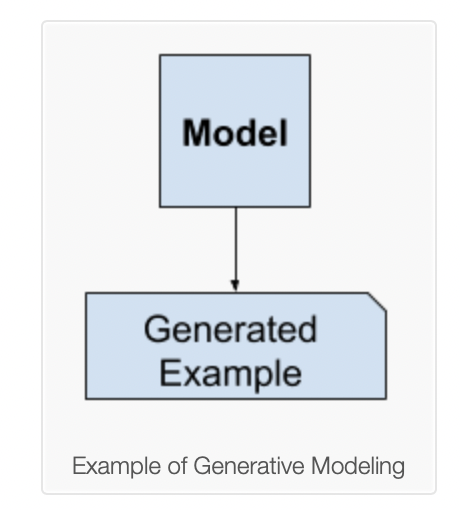
\includegraphics[width=\linewidth,height=7cm]{figures/3.png}
    \caption{ Example of generative modeling}
    \label{fig:GAN model}
\end{figure}



	\begin{figure}[h!]
    \centering
    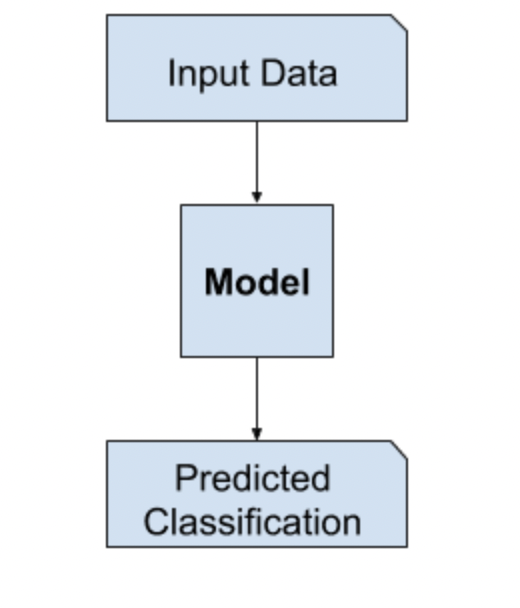
\includegraphics[width=\linewidth,height=7cm]{figures/4.png}
    \caption{  Example of discriminate modeling}
    \label{fig:GAN model}
\end{figure}


	\begin{figure}[h!]
    \centering
    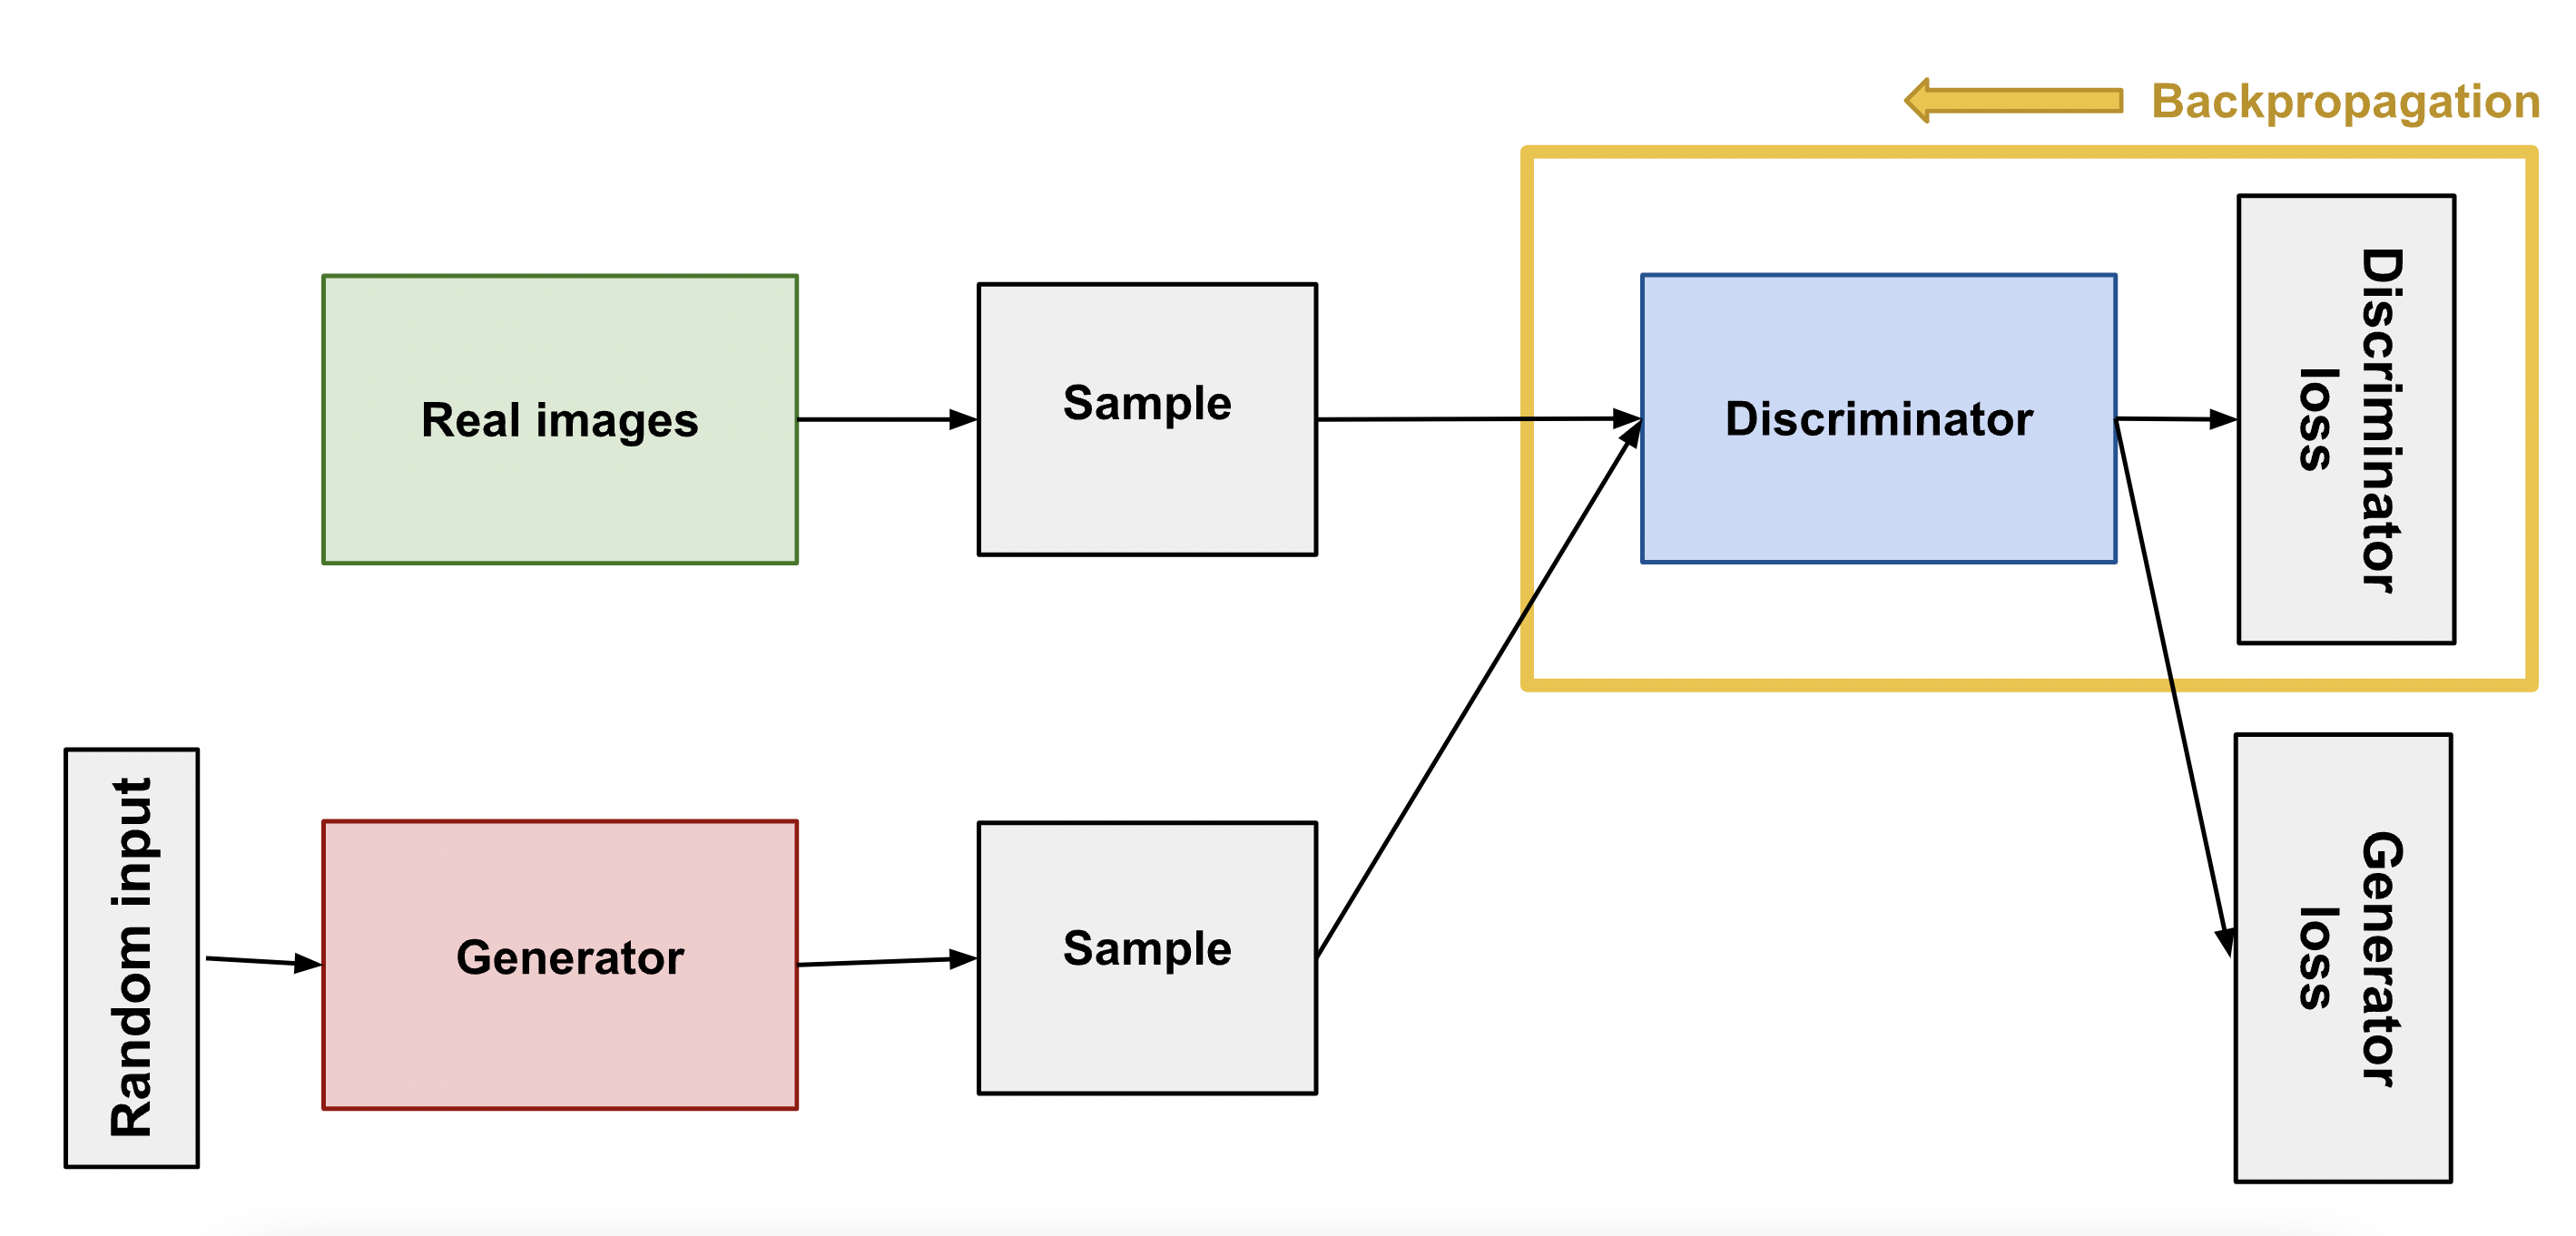
\includegraphics[width=\linewidth,height=7cm]{figures/1.png}
    \caption{ Architecture of GAN model}
    \label{fig:GAN model}
\end{figure}



\par  

\chapter{Motivation} \label{ch:background}
\subsection{Objective}

\par Satellite photographs can be translated to map images using the GAN model. Conditional adversarial networks are being studied as a broad solution to image-to-image translation problems.



\subsection{Motivation}
\par GANs are used in the conditional circumstance. In the same way as GANs learn a generative model of data, conditional GANs (cGANs) train a conditional generative model. As a result, convolutional neural networks (cGANs) are well-suited to image-to-image translation tasks, where we condition on an input image and produce a corresponding output image.
GANs have garnered a lot of attention in the previous two years, and many of the solutions we look at in this paper have already been described. Previous research focused on specific applications, thus it's uncertain how useful image-conditional GANs can be as a general-purpose solution for image-to-image translation. Our key contribution is to demonstrate that conditional GANs produce reasonable results for a variety of problems.

\chapter{Literature Review} \label{ch:Objective}

 \textbf  {[1] Deep Hashing Based on VAE-GAN for Efficient Similarity Retrieval}

In this research, a VAE-GAN based hashing architecture for fast photo retrieval was investigated. The method combines a Variational autoencoder (VAE) with a Generative adversarial network to generate content-preserving pictures for pairwise hashing learning (GAN). Accepting actual and synthesised images in paired form, an adversarial generative approach is utilised to learn a semantic perserving feature mapping model.
Each pairwise image feature vector is converted to hash codes, which are subsequently used in a pairwise ranking loss to maintain relative image similarity. TensorFlow, one of the most widely used deep learning frameworks, should be utilised to implement VGH. All of the weights are set up by xavier. In the midst of putting together an image. On Adam, the VAE-GAN models are trained on all datasets.

 \textbf { [2] Recurrent Topic Transition GAN for Visual Paragraph Generation}
 
The RTT-GAN (Recurrent Topic Transition Generative Adversarial Network) that has been proposed builds an adversarial framework between a structured paragraph generator and multi-level paragraph discriminators.
To create sentences frequently, the paragraph generator uses region-based visual and language attention strategies at each level. Multi-level adversarial discriminators assess the quality of generated paragraph.sentences on two levels: sentence plausibility and paragraph topic-transition coherence.


 \textbf {[3] Natural Language Processing approaches for Text2Image using Machine Learning Algorithms}

A word cloud was used in this research report to help the reader understand the artist's concept. MLA - Random Forest was also used, with a classification accuracy of 78 on the dataset in question. Transform the data source Creating an image from text data The morphological stage is the first and is concerned with the various forms of words. Syntactical analysis will focus on the various relationships between the words in the sentence in the next stage. We'll move on to semantics when we've mastered some synthetic structures. As a result, semantics is concerned with figuring out what something means. The highest level of abstraction is pragmatics, which is the ultimate stage.




 \textbf {[4] Image-to-Image Translation with Conditional Adversarial Networks}

\par Demonstrate that, among other things, the GAN approach can be used to synthesise photos from label maps, reconstruct objects from edge maps, and colourize images. According to the findings of this research, conditional adversarial networks appear to be a promising answer for many image-to-image translation difficulties, particularly those involving highly organised graphical outputs. These networks learn a loss that is specific to the task and data, making them effective in a variety of scenarios.




\chapter{Methodology } \label{ch:literature_review}
\subsection{ Methodology}

GANs are generative models that learn a mapping from random noise vector z to output image y, G : z → y. In 

	\begin{figure}[h!]
     \centering
    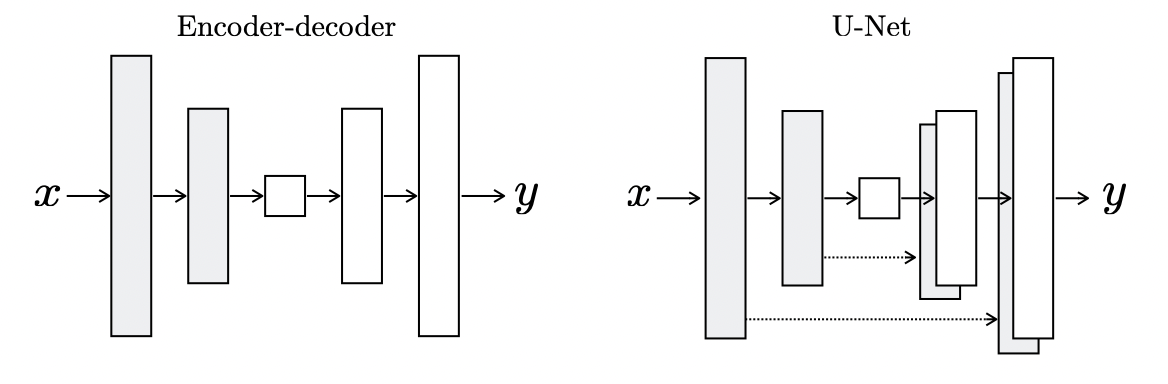
\includegraphics[width=\linewidth,height=7cm]{figures/5.png}
    \caption{ Two choices for the architecture of the generator. The “U-Net” is an encoder-decoder with skip connections between mirrored layers in the encoder and decoder stacks }
    \label{fig:GAN model}

\end{figure}

\subsection{Network architectures}

The architectures of our generator and discriminator are based on those in. Convolution-BatchNorm-ReLu modules are used by both the generator and the discriminator.

\subsection{Generator with skips}

The mapping of a high resolution input grid to a high resolution output grid is a distinguishing property of image-to-image translation difficulties. Furthermore, the input and output for the problems we analyse have different surface appearances, but they are both renderings of the same underlying structure. As a result, the input structure is closely aligned with the output structure. The generator architecture is based on these concepts.

\par An encoder-decoder network has been employed in several past solutions to difficulties in this field. The input is transmitted through a series of layers that gradually downsample the data until it reaches a bottleneck layer, when the process is reversed. All information flow must pass through all layers, including the bottleneck, in such a network. There is a lot of low-level information shared between the input and output for many picture translation difficulties, and it would be preferable to send this information directly across the network. In image colorization, for example, the input and output share the location of prominent edges.


\par We add skip connections, which follow the general shape of a "U-Net," to provide the generator a way to get around the bottleneck for information like this. We add skip connections between each layer I and layer n I where n is the total number of layers, in particular. Each skip connection simply concatenates all layer I channels with layer n-i channels.

\subsection{Markovian discriminator (PatchGAN)}

On image production challenges, it is generally known that the L2 loss and L1 generate hazy outcomes. Although these losses may not promote high-frequency sharpness, they do, in many circumstances, accurately capture low frequencies. We don't need a totally new system to enforce accuracy at low frequencies for cases when this is the case. L1 is sufficient.

This justifies using an L1 term to force low-frequency accuracy by confining the GAN discriminator to exclusively simulate high-frequency structure. It is sufficient to limit our attention to the structure in local image patches in order to represent high-frequencies. As a result, we create a PatchGAN, a discriminator architecture that only penalises structure at the patch size. This discriminator attempts to determine whether each of an image's N N patches is authentic or phoney. We convolutionally run this discriminator across the image, average all responses to get the final output of D.

We show that N can be substantially smaller than the image's full size while still producing high-quality results. This is beneficial since a smaller PatchGAN has less parameters, runs faster, and can process images of any size.
A discriminator like this effectively represents the image as a Markov random field, assuming that pixels separated by more than a patch diameter are independent. This link was previously investigated in, and it is also a prevalent assumption in texture and style models. As a result, our PatchGAN can be viewed as a texture/style loss.

\subsection{Optimization and inference}

\par We use the traditional strategy of alternating between one gradient descent step on D and one step on G to improve our networks. Rather than training G to minimise log(1 D(x, G(x, z)), we train it to maximise log D(x, G(x, z) as indicated in the original GAN study. In addition, we divide the goal by two while optimising D, which reduces D's learning rate compared to G's. With a learning rate of 0.0002, and momentum parameters 1 = 0.5, 2 = 0.999, we employ minibatch SGD and the Adam solver.

\par At inference time, we run the generator net in the same way that we did during training. This differs from the standard technique in that we apply dropout at test time and batch normalisation using the test batch's statistics rather than the training batch's aggregated data. When the batch size is set to 1, this method of batch normalising is known as "instance normalisation," and it has been shown to be effective in picture production jobs. Depending on the experiment, we utilise batch sizes ranging from one to ten.



%\chapter{Main Topic 2} \label{ch:main_chapter2}
%\section{Dataset}


Aerial photograph of maps 1096 training pictures collected from Google Maps, trained for 200 epochs with random jitter and mirroring, batch size 1, and random jitter. Images were collected from all throughout New York City. The data was then divided into train and test groups based on the sampling region's median latitude (with a buffer region added to ensure that no training pixel appeared in the test set). There are 1096 photos in the train dataset and 1098 images in the validation dataset.


%

%\chapter{Research Work} \label{ch:proposal}
%\section{Dataset}


Aerial photograph of maps 1096 training pictures collected from Google Maps, trained for 200 epochs with random jitter and mirroring, batch size 1, and random jitter. Images were collected from all throughout New York City. The data was then divided into train and test groups based on the sampling region's median latitude (with a buffer region added to ensure that no training pixel appeared in the test set). There are 1096 photos in the train dataset and 1098 images in the validation dataset.




\chapter{Dataset Description} \label{ch:main_chapter2}
\section{Dataset}


Aerial photograph of maps 1096 training pictures collected from Google Maps, trained for 200 epochs with random jitter and mirroring, batch size 1, and random jitter. Images were collected from all throughout New York City. The data was then divided into train and test groups based on the sampling region's median latitude (with a buffer region added to ensure that no training pixel appeared in the test set). There are 1096 photos in the train dataset and 1098 images in the validation dataset.


%
\chapter{ Dataset Analysis } \label{ch:experimental_results}
\section{Data analysis}


discriminator_model.py 
import torch
import torch.nn as nn


class CNNBlock(nn.Module):
    def __init__(self, in_channels, out_channels, stride):
        super(CNNBlock, self).__init__()
        self.conv = nn.Sequential(
            nn.Conv2d(
                in_channels, out_channels, 4, stride, 1, bias=False, padding_mode="reflect"
            ),
            nn.BatchNorm2d(out_channels),
            nn.LeakyReLU(0.2),
        )

    def forward(self, x):
        return self.conv(x)


class Discriminator(nn.Module):
    def __init__(self, in_channels=3, features=[64, 128, 256, 512]):
        super().__init__()
        self.initial = nn.Sequential(
            nn.Conv2d(
                in_channels * 2,
                features[0],
                kernel_size=4,
                stride=2,
                padding=1,
                padding_mode="reflect",
            ),
            nn.LeakyReLU(0.2),
        )

        layers = []
        in_channels = features[0]
        for feature in features[1:]:
            layers.append(
                CNNBlock(in_channels, feature, stride=1 if feature == features[-1] else 2),
            )
            in_channels = feature

        layers.append(
            nn.Conv2d(
                in_channels, 1, kernel_size=4, stride=1, padding=1, padding_mode="reflect"
            ),
        )

        self.model = nn.Sequential(*layers)

    def forward(self, x, y):
        x = torch.cat([x, y], dim=1)
        x = self.initial(x)
        x = self.model(x)
        return x


def test():
    x = torch.randn((1, 3, 256, 256))
    y = torch.randn((1, 3, 256, 256))
    model = Discriminator(in_channels=3)
    preds = model(x, y)
    print(model)
    print(preds.shape)


if __name__ == "__main__":
    test()

requirements.txt
albumentations==1.1.0
certifi==2020.6.20
colorama==0.4.4
cycler==0.11.0
decorator==4.4.2
imageio==2.13.1
joblib==1.1.0
kiwisolver==1.3.1
matplotlib==3.3.4
networkx==2.5.1
numpy==1.19.5
opencv-python-headless==4.5.4.60
Pillow==8.4.0
pyparsing==3.0.6
python-dateutil==2.8.2
PyWavelets==1.1.1
PyYAML==6.0
qudida==0.0.4
scikit-image==0.17.2
scikit-learn==0.24.2
scipy==1.5.4
six==1.16.0
threadpoolctl==3.0.0
tifffile==2020.9.3
torch==1.10.0
torchvision==0.11.1
tqdm==4.62.3
typing_extensions==4.0.1
wincertstore==0.2


generator_model.py 

import torch
import torch.nn as nn


class Block(nn.Module):
    def __init__(self, in_channels, out_channels, down=True, act="relu", use_dropout=False):
        super(Block, self).__init__()
        self.conv = nn.Sequential(
            nn.Conv2d(in_channels, out_channels, 4, 2, 1, bias=False, padding_mode="reflect")
            if down
            else nn.ConvTranspose2d(in_channels, out_channels, 4, 2, 1, bias=False),
            nn.BatchNorm2d(out_channels),
            nn.ReLU() if act == "relu" else nn.LeakyReLU(0.2),
        )

        self.use_dropout = use_dropout
        self.dropout = nn.Dropout(0.5)
        self.down = down

    def forward(self, x):
        x = self.conv(x)
        return self.dropout(x) if self.use_dropout else x


class Generator(nn.Module):
    def __init__(self, in_channels=3, features=64):
        super().__init__()
        self.initial_down = nn.Sequential(
            nn.Conv2d(in_channels, features, 4, 2, 1, padding_mode="reflect"),
            nn.LeakyReLU(0.2),
        )
        self.down1 = Block(features, features * 2, down=True, act="leaky", use_dropout=False)
        self.down2 = Block(
            features * 2, features * 4, down=True, act="leaky", use_dropout=False
        )
        self.down3 = Block(
            features * 4, features * 8, down=True, act="leaky", use_dropout=False
        )
        self.down4 = Block(
            features * 8, features * 8, down=True, act="leaky", use_dropout=False
        )
        self.down5 = Block(
            features * 8, features * 8, down=True, act="leaky", use_dropout=False
        )
        self.down6 = Block(
            features * 8, features * 8, down=True, act="leaky", use_dropout=False
        )
        self.bottleneck = nn.Sequential(
            nn.Conv2d(features * 8, features * 8, 4, 2, 1), nn.ReLU()
        )

        self.up1 = Block(features * 8, features * 8, down=False, act="relu", use_dropout=True)
        self.up2 = Block(
            features * 8 * 2, features * 8, down=False, act="relu", use_dropout=True
        )
        self.up3 = Block(
            features * 8 * 2, features * 8, down=False, act="relu", use_dropout=True
        )
        self.up4 = Block(
            features * 8 * 2, features * 8, down=False, act="relu", use_dropout=False
        )
        self.up5 = Block(
            features * 8 * 2, features * 4, down=False, act="relu", use_dropout=False
        )
        self.up6 = Block(
            features * 4 * 2, features * 2, down=False, act="relu", use_dropout=False
        )
        self.up7 = Block(features * 2 * 2, features, down=False, act="relu", use_dropout=False)
        self.final_up = nn.Sequential(
            nn.ConvTranspose2d(features * 2, in_channels, kernel_size=4, stride=2, padding=1),
            nn.Tanh(),
        )

    def forward(self, x):
        d1 = self.initial_down(x)
        d2 = self.down1(d1)
        d3 = self.down2(d2)
        d4 = self.down3(d3)
        d5 = self.down4(d4)
        d6 = self.down5(d5)
        d7 = self.down6(d6)
        bottleneck = self.bottleneck(d7)
        up1 = self.up1(bottleneck)
        up2 = self.up2(torch.cat([up1, d7], 1))
        up3 = self.up3(torch.cat([up2, d6], 1))
        up4 = self.up4(torch.cat([up3, d5], 1))
        up5 = self.up5(torch.cat([up4, d4], 1))
        up6 = self.up6(torch.cat([up5, d3], 1))
        up7 = self.up7(torch.cat([up6, d2], 1))
        return self.final_up(torch.cat([up7, d1], 1))


def test():
    x = torch.randn((1, 3, 256, 256))
    model = Generator(in_channels=3, features=64)
    preds = model(x)
    print(preds.shape)


if __name__ == "__main__":
    test()




Train.py
import torch
from utils import save_checkpoint, load_checkpoint, save_some_examples
import torch.nn as nn
import torch.optim as optim
import os
os.environ["KMP_DUPLICATE_LIB_OK"]="TRUE"

import config
from dataset import MapDataset
from generator_model import Generator
from discriminator_model import Discriminator
from torch.utils.data import DataLoader
from tqdm import tqdm
from torchvision.utils import save_image

torch.backends.cudnn.benchmark = True


def train_fn(
    disc, gen, loader, opt_disc, opt_gen, l1_loss, bce, g_scaler, d_scaler,
):
    loop = tqdm(loader, leave=True)

    for idx, (x, y) in enumerate(loop):
        x = x.to(config.DEVICE)
        y = y.to(config.DEVICE)

        # Train Discriminator
        with torch.cuda.amp.autocast():
            y_fake = gen(x)
            D_real = disc(x, y)
            D_real_loss = bce(D_real, torch.ones_like(D_real))
            D_fake = disc(x, y_fake.detach())
            D_fake_loss = bce(D_fake, torch.zeros_like(D_fake))
            D_loss = (D_real_loss + D_fake_loss) / 2

        disc.zero_grad()
        d_scaler.scale(D_loss).backward()
        d_scaler.step(opt_disc)
        d_scaler.update()

        # Train generator
        with torch.cuda.amp.autocast():
            D_fake = disc(x, y_fake)
            G_fake_loss = bce(D_fake, torch.ones_like(D_fake))
            L1 = l1_loss(y_fake, y) * config.L1_LAMBDA
            G_loss = G_fake_loss + L1

        opt_gen.zero_grad()
        g_scaler.scale(G_loss).backward()
        g_scaler.step(opt_gen)
        g_scaler.update()

        if idx % 10 == 0:
            loop.set_postfix(
                D_real=torch.sigmoid(D_real).mean().item(),
                D_fake=torch.sigmoid(D_fake).mean().item(),
            )


def main():
    disc = Discriminator(in_channels=3).to(config.DEVICE)
    gen = Generator(in_channels=3, features=64).to(config.DEVICE)
    opt_disc = optim.Adam(disc.parameters(), lr=config.LEARNING_RATE, betas=(0.5, 0.999),)
    opt_gen = optim.Adam(gen.parameters(), lr=config.LEARNING_RATE, betas=(0.5, 0.999))
    BCE = nn.BCEWithLogitsLoss()
    L1_LOSS = nn.L1Loss()

    if config.LOAD_MODEL:
        load_checkpoint(
            config.CHECKPOINT_GEN, gen, opt_gen, config.LEARNING_RATE,
        )
        load_checkpoint(
            config.CHECKPOINT_DISC, disc, opt_disc, config.LEARNING_RATE,
        )

    train_dataset = MapDataset(root_dir=config.TRAIN_DIR)
    train_loader = DataLoader(
        train_dataset,
        batch_size=config.BATCH_SIZE,
        shuffle=True,
        num_workers=config.NUM_WORKERS,
    )
    g_scaler = torch.cuda.amp.GradScaler()
    d_scaler = torch.cuda.amp.GradScaler()
    val_dataset = MapDataset(root_dir=config.VAL_DIR)
    val_loader = DataLoader(val_dataset, batch_size=1, shuffle=False)

    for epoch in range(config.NUM_EPOCHS):
        train_fn(
            disc, gen, train_loader, opt_disc, opt_gen, L1_LOSS, BCE, g_scaler, d_scaler,
        )

        if config.SAVE_MODEL and epoch % 5 == 0:
            save_checkpoint(gen, opt_gen, filename=config.CHECKPOINT_GEN)
            save_checkpoint(disc, opt_disc, filename=config.CHECKPOINT_DISC)

        save_some_examples(gen, val_loader, epoch, folder="evaluation")


if __name__ == "__main__":
    main()


Utils.py
import torch
import config
from torchvision.utils import save_image

def save_some_examples(gen, val_loader, epoch, folder):
    x, y = next(iter(val_loader))
    x, y = x.to(config.DEVICE), y.to(config.DEVICE)
    gen.eval()
    with torch.no_grad():
        y_fake = gen(x)
        y_fake = y_fake * 0.5 + 0.5  # remove normalization#
        save_image(y_fake, folder + f"/y_gen_{epoch}.png")
        save_image(x * 0.5 + 0.5, folder + f"/input_{epoch}.png")
        if epoch == 1:
            save_image(y * 0.5 + 0.5, folder + f"/label_{epoch}.png")
    gen.train()


def save_checkpoint(model, optimizer, filename="my_checkpoint.pth.tar"):
    print("=> Saving checkpoint")
    checkpoint = {
        "state_dict": model.state_dict(),
        "optimizer": optimizer.state_dict(),
    }
    torch.save(checkpoint, filename)


def load_checkpoint(checkpoint_file, model, optimizer, lr):
    print("=> Loading checkpoint")
    checkpoint = torch.load(checkpoint_file, map_location=config.DEVICE)
    model.load_state_dict(checkpoint["state_dict"])
    optimizer.load_state_dict(checkpoint["optimizer"])

    # If we don't do this then it will just have learning rate of old checkpoint
    # and it will lead to many hours of debugging \:
    for param_group in optimizer.param_groups:
        param_group["lr"] = lr
        




\subsection{Data Preprocessing}




\chapter{Results and Discussion}\label{ch:main_chapter5}
\subsection{Results and Discussion}
In 
\chapter{Conclusion and Future Work} \label{ch:Conclusion}
\subsection{Conclusion and Future Work}
 In this




\printbibliography
\end{document}          
